\documentclass[11pt,a4paper]{article}
\usepackage[a4paper,margin=22mm,headheight=14pt]{geometry}
\usepackage{fontspec}
\IfFontExistsTF{DejaVu Sans Mono}{\setmonofont{DejaVu Sans Mono}}{}
\usepackage{amsmath,amssymb,booktabs,tabularx}
\usepackage{graphicx,tikz,fancyvrb,fancyhdr,microtype}
\usetikzlibrary{arrows.meta}
\usepackage[hidelinks]{hyperref}
\setlength{\emergencystretch}{2em}
\pagestyle{fancy}
\fancyhf{}
\fancyhead[L]{Meta-Synset and Invariant: Typed Revision of Representations (v2.4)}
\fancyhead[R]{A. Strand}
\fancyfoot[C]{\thepage}
\title{Meta-Synset and Invariant: A Typed System for Revising Research Representations\\[0.7em]
\large The Duality of Expansion and Narrowing, the Algebra of the Residual Gap \(\Delta(T)\), Dependent Inference Licenses, and a Machine-Verified Kernel in Lean 4.36.0}
\author{Aleksandr Strand}
\date{23 November 2026\\[0.3em]\small Preprint v2.4. Manuscript with the v2.4 kernel and Axis 2\\(Gates 14--16 v2.4) verified in Lean 4.36.0}
\begin{document}
\maketitle
\begin{abstract}

Research search has two modes with incompatible requirements. Generating candidates through cross-domain analogies requires controlled conceptual drift, whereas proof-based verification and the choice of the next experiment require referential transparency and prohibit retroactive changes to definitions. We formalize a dual architecture for the hypothesis language \(L_H\): meta-synset (focused expansion) and invariant (strict narrowing). The two circuits are linked by the Freeze phase transition, typed transfer via CertifiedTransfer with a mandatory residual gap \(\Delta(T)=R\setminus S_{\rm ok}\), and the branching step StepBranch. Compared with v1.0, three structural defects of naive scope indexing are addressed: (1) DirectEvidence s A c is tied to the particular claim \(c:\mathrm{Claim}\,s\) through \(\mathrm{Denote}:\mathrm{Claim}\,s\to\mathrm{Prop}\); (2) covered and total justifications are indexed by a pointwise-dependent family \(c:Q\to\mathrm{Claim}\,s\), so evidenceAt can be constructed pointwise without assuming a nonempty request, and pointwise\_\allowbreak unproved\_\allowbreak blocks\_\allowbreak any\_\allowbreak total precludes bypassing the completion bridge when a requested claim is false under the premises; and (3) the cross-scope lift liftScope uses a conditional ScopeBridge, valid only on ModelOk, and explicitly leaves a model gap ModelGap. A dependent inference license \(\kappa:\mathrm{Judgement}(\alpha,\delta)\) is introduced with soundness, language restriction (restriction\_\allowbreak sound), and anti-leakage results. For the StepBranch probe, a full SymbolLift is sufficient, and neither binPreserving nor injectiveBin can be dropped in general.

The second axis of escalation, Axis 2 (Gates 14–16), is also formalized and verified: escalation of the observation port using a gauge-equivalence certificate GaugeEquivCert and exclusion of observationally unproductive hidden extensions (Gate 14); an intervention algebra with a computable control mask \(K\) and commutator \([T_L,T_R]\) under a normalizer \(N\) (Gate 15); and a quantitative residual gap \(\Delta_\varepsilon\) (HasGapBound) and product certificates for two independent e-values at a fixed horizon of two on exact discrete measures (Gate 16). All 44 key declarations across four modules were machine-verified in a single Lean 4.36.0 run (0 errors, 0 warnings, 0 sorryAx). Of these, 23 have no axiom dependencies; the others use only propext, Classical.choice and Quot.sound. Twelve additional Gate 11–12 v12.3 theorems were verified in [2].

\end{abstract}
\section{The problem of two incompatible modes of scientific search}

Formal identification theory and proof-based representational change [2, 10] operate within a given structure. With a fixed object language \(L=(G,J_G)\), observations \(D\), and the semantic version space
\[
\mathcal V(L,D)=\{f\in B(L):\forall (x,y)\in D,\ f(x)=y\},\qquad B(L)=\operatorname{im}J_G, \tag{1}
\]
one can define consistency, unique identification \(|\mathcal V(L,D)|=1\), the agreement set \(\operatorname{Agree}(\mathcal V)\), and one-step elimination of a language, \(\mathcal V(L,D\cup\{(q,y)\})=\varnothing\). But once the old language has been refuted, or before a conceptual frame has fully formed, the researcher faces two competing requirements.

\begin{enumerate}
\item \textbf{Expansion.} Breaking conceptual fixation and finding a nontrivial replacement class (for example, moving from counter memory to a stack or queue) requires comparing objects from distant domains under a deliberately incomplete preliminary lens \(\lambda_t\), allowing conceptual boundaries to shift and split.
\item \textbf{Strict narrowing.} To prevent the comparison of candidates, rejection of alternatives, and choice of the next experiment from becoming retroactive adjustment, each claim must be frozen with its version, scope, and premises. Evidence must be kept separate from any desired but unproved generalization.

\end{enumerate}
Mixing the two modes yields two symmetric pathologies: requiring final proofs at generation time traps the search among synonyms in one domain; allowing floating definitions during verification produces degenerative drift. The meta-synset \(\leftrightarrow\) invariant architecture puts the modes in two isolated circuits of \(L_H\), linked at exactly one typed seam, the Freeze phase transition (Figure 1).

\begin{figure}[htbp]
\centering
\resizebox{\linewidth}{!}{%
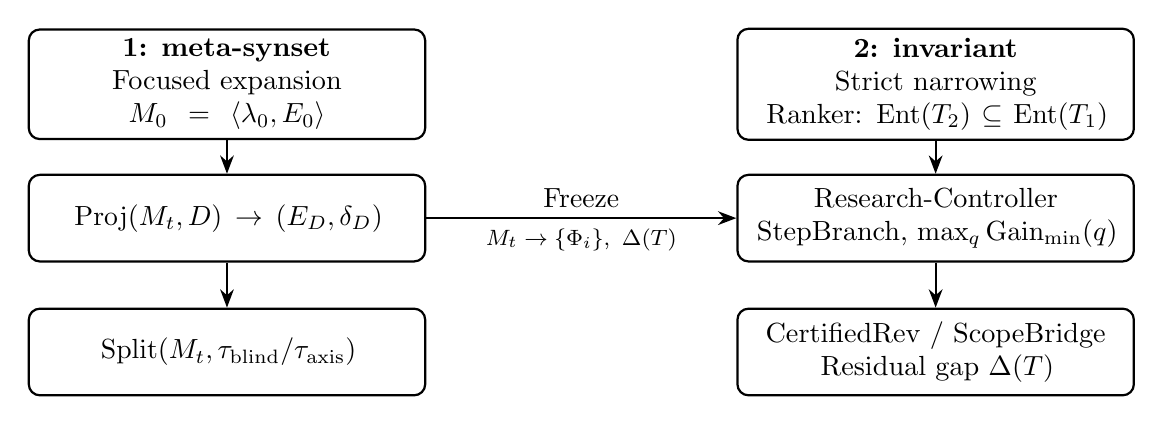
\begin{tikzpicture}[>=Stealth, box/.style={draw,rounded corners,align=center,minimum height=11mm,text width=48mm}, thick]
\node[box] (m) at (0,0) {\textbf{1: meta-synset}\\Focused expansion\\\(M_0=\langle\lambda_0,E_0\rangle\)};
\node[box] (p) at (0,-1.7) {\(\mathrm{Proj}(M_t,D)\to(E_D,\delta_D)\)};
\node[box] (s) at (0,-3.4) {\(\mathrm{Split}(M_t,\tau_{\mathrm{blind}}/\tau_{\mathrm{axis}})\)};
\node[box] (r) at (9,0) {\textbf{2: invariant}\\Strict narrowing\\Ranker: \(\mathrm{Ent}(T_2)\subseteq\mathrm{Ent}(T_1)\)};
\node[box] (c) at (9,-1.7) {Research-Controller\\StepBranch, \(\max_q\operatorname{Gain}_{\min}(q)\)};
\node[box] (b) at (9,-3.4) {CertifiedRev / ScopeBridge\\Residual gap \(\Delta(T)\)};
\draw[->] (m)--(p); \draw[->] (p)--(s);
\draw[->] (r)--(c); \draw[->] (c)--(b);
\draw[->] (p)--node[above]{Freeze} node[below,font=\footnotesize]{\(M_t\to\{\Phi_i\},\ \Delta(T)\)} (c);
\end{tikzpicture}}
\caption{Dual architecture. A drifting operand \(M_t\) cannot enter the Ranker directly: the Freeze phase transition ends the drift and records the residual gap \(\Delta(T)\).}
\end{figure}

\section{Meta-synset: focused expansion and controlled drift}

Unlike an ordinary synset (as in WordNet), which groups synonyms within one subject layer, a meta-synset accumulates structural analogues from different domains in a controlled way, bringing them to a bifurcation point where hidden axes of difference become visible [1].

\textbf{Definition 2.1 (Meta-synset and internal tuple).} Let \(U=\bigsqcup_{d\in D}\mathrm{Obj}_d\) be the tagged disjoint union of domain objects. The preliminary lens of version \(t\) is a partial selection procedure \(\lambda_t:U\rightharpoonup\mathcal P(\mathrm{Pred})\). It must be able to return “not applicable” without choosing new features after seeing the result. The version-\(t\) meta-synset operand is \(M_t=\langle\lambda_t,E_t\rangle\), where \(|\operatorname{domains}(M_t)|\ge2\). Within \(M_t\), an evidence tuple has coordinates
\[
e=(d,I,s^-,s^+,u,K,\alpha,\delta,\kappa),\tag{2}
\]
where \(I=(X,Y,Z,B)\) specifies the interface and budget, \(u:s^-\mapsto s^+\) is an admissible operation, \(K\) marks coordinates as held, changed, or uncontrolled, \(\alpha=(a,b,c,\eta)\) is a structural map, \(\delta\) lists lost or unverified properties, and \(\kappa\) is the dependent inference license (Section~5).

All changes to the operand proceed through typed operators:

\begin{itemize}
\item \(\mathrm{Proj}(M_t,D)\to(E_D,\delta_D)\) projects the lens \(\lambda_t\) into a new domain \(D\), applies an anti-synonym filter, and immediately records lost features \(\delta_D\).
\item \(\mathrm{Split}(M_t,\tau_{\rm blind})\to M_{t+1}\) excludes an off-axis counterexample without splitting the operand.
\item \(\mathrm{Split}(M_t,\tau_{\rm axis})\to(M^a_{t+1},M^b_{t+1})\) uses an axial test that holds one hidden axis fixed and breaks another; it closes \(M_t\) and opens two new branches.
\item \(\mathrm{Merge}(M_1,M_2)\to M_{12}\) requires compatible lenses and agreement of the extracted structures on shared domains.
\item \(\mathrm{Freeze}(M_t)\to\{\Phi_1,\ldots,\Phi_k\}\) ends the drift and outputs frozen candidates \(\Phi=(P,S,A,\bot_\Phi)\).

\end{itemize}
Expansion is governed by three axioms: referential transparency (the status of \(M_{t+1}\) does not transfer to \(M_t\)), nondegeneracy (\(|\operatorname{domains}(M_t)|\ge2\)), and closure at bifurcation (\(M_t\) closes after an axial split). Two operational boundaries are also explicit: the phase boundary between \(M_t\) and \(\Phi\), and the limit of reproducibility across observers. For example, start with \(M_0=\langle\lambda_{\rm filter},\{\text{firewall, cell membrane, customs checkpoint}\}\rangle\). After projecting into neural networks (\(\delta\): “the physical barrier is lost”) and excluding a brick wall as an off-axis counterexample, the axial test “Markov blanket” yields two independent branches: \(M_{2a}\) (interface shielding) and \(M_{2b}\) (selective rule-based filtering). Only then does \(\mathrm{Freeze}(M_{2b})\) pass frozen candidates to invariant. The current Lean kernel mechanizes the basic meta-synset operations (MetaOperand, metaProj, metaFreeze). Full Split/Merge semantics and the seven Ranker axes remain formal specifications.

\section{Invariant: a partial order of consequences and a probe controller}

The invariant circuit answers two questions that meta-synset does not: what exactly is established (Ranker), and which experiment to run next (Research-Controller).

\textbf{Separating the evidence carrier from its content.} The carrier (manual derivation, Lean kernel term, finite certificate, exhaustive enumeration, or empirical protocol) does not automatically determine the strength of the conclusion. A LeanKernelTerm may prove a property over four finite histories or a universal theorem on \(\Sigma^*\) [1]. The Ranker therefore assesses candidates along seven axes (Proof, Scope, Robustness, Causality, Transfer, Utility, and Discrimination) without imposing an aggregate score. It uses the dominance preorder \(T_1\succeq T_2\iff\operatorname{Ent}(T_2)\subseteq\operatorname{Ent}(T_1)\) and four comparison outcomes: dominates, is dominated, incomparable, or insufficient information. The standing of a claim is strictly separated from the research queue: a weak hypothesis with a cheap decisive counterexample goes to the front of the Research-Controller's queue.

\section{The topology of scopes, sealed evidence, and the algebra of the gap \(\Delta(T)\)}

The linking object CertifiedTransfer (Section~1) is implemented in the kernel by TransferCoverage and CoveredJustification. The covering partition \(R(q)\to S_{\rm ok}(q)\lor \mathrm{Gap}(q)\) guarantees
\[
\Delta(T)=R\setminus S_{\rm ok}\subseteq\{q\in R:\mathrm{Gap}(q)\}.
\]
Equality requires a separate condition that \(S_{\rm ok}\) and Gap be disjoint; GapEmpty Gap implies \(\Delta(T)=\varnothing\).

In the original v1.0 design, indexing by Scope alone let one claim be substituted for another within a scope and let a nonempty gap be hidden during Lift. The v2.1 kernel separated CoveredJustification and TotalJustification, but the claim \(c:\mathrm{Claim}\,s\) was still constant over \(Q\). A nonempty gap therefore blocked bridgeComplete but did not prevent constructing a TotalJustification directly. The verified v2.4 kernel (epistemic\_\allowbreak revision\_\allowbreak kernel\_\allowbreak v2\_\allowbreak 4.lean) addresses this by indexing claims pointwise, \(c:Q\to\mathrm{Claim}\,s\).

\textbf{The topology of the four scopes.} Claims are divided into four disjoint scopes: FinitePrefix (a finite prefix of the append-only RawLog); LanguageMenu (a finite menu \(R\) of alternatives frozen before the experiment); InfiniteLanguage (the full infinite set of words \(\Sigma^*\)); and RevisionSpace (the space of traces and revision layers \(\Delta_L/\Delta_D/\Delta_\pi\)).

\textbf{Listing 1.} The verified v2.4 kernel (Lean 4.36.0): pointwise-dependent claims \(c:Q\to\mathrm{Claim}\,s\), pointwise evidenceAt, and conditional ScopeBridge.

\begin{Verbatim}[fontsize=\small]
structure CoveredJustification (Q : Type) (s : Scope) (A : Premise)
    (c : Q → Claim s) where
  R          : Q → Prop
  Covered    : Q → Prop
  Gap        : Q → Prop
  partition  : ∀ q : Q, R q → Covered q ∨ Gap q
  localProof : A → ∀ q : Q, Covered q → Denote (c q)

\end{Verbatim}
\begin{Verbatim}[fontsize=\small]
structure TotalJustification (Q : Type) (s : Scope) (A : Premise)
    (c : Q → Claim s) where
  R          : Q → Prop
  evidenceAt : ∀ q : Q, R q → DirectEvidence s A (c q)
  fullCover  : A → ∀ q : Q, R q → Denote (c q)

\end{Verbatim}
\begin{Verbatim}[fontsize=\small]
structure ScopeBridge (Q2 : Type) (s1 s2 : Scope) (A1 A2 : Premise)
    (c1 : Claim s1) (c2 : Q2 → Claim s2) (ModelOk : Q2 → Prop) where
  liftProof : A2 → Denote c1 → ∀ q : Q2, ModelOk q → Denote (c2 q)

\end{Verbatim}
\begin{figure}[htbp]
\centering
\resizebox{\linewidth}{!}{%
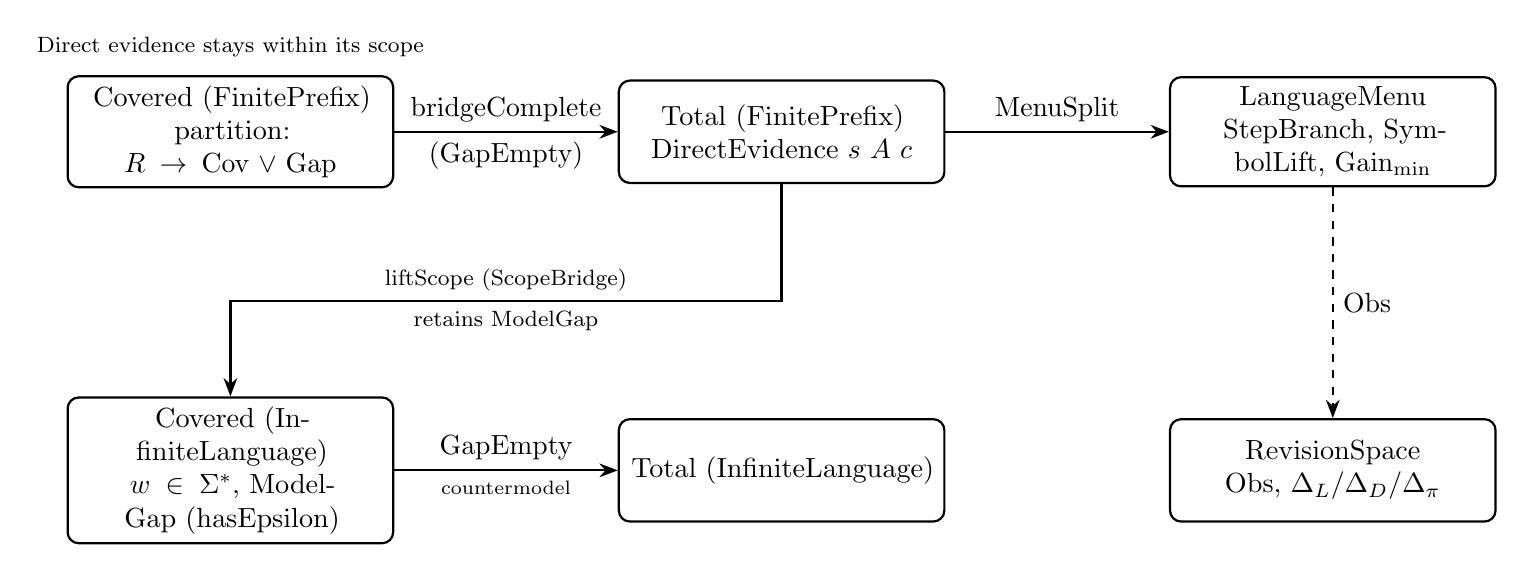
\begin{tikzpicture}[>=Stealth, box/.style={draw,rounded corners,align=center,minimum height=13mm,text width=39mm}, thick]
\node[box] (a) at (0,0) {Covered (FinitePrefix)\\partition: \(R\to\mathrm{Cov}\lor\mathrm{Gap}\)};
\node[box] (b) at (7,0) {Total (FinitePrefix)\\DirectEvidence \(s\ A\ c\)};
\node[box] (c) at (14,0) {LanguageMenu\\StepBranch, SymbolLift, \(\mathrm{Gain}_{\min}\)};
\node[box] (d) at (0,-4.3) {Covered (InfiniteLanguage)\\\(w\in\Sigma^*\), ModelGap (hasEpsilon)};
\node[box] (e) at (7,-4.3) {Total (InfiniteLanguage)};
\node[box] (f) at (14,-4.3) {RevisionSpace\\Obs, \(\Delta_L/\Delta_D/\Delta_\pi\)};
\draw[->] (a)--node[above]{bridgeComplete} node[below]{(GapEmpty)} (b);
\draw[->] (b)--node[above]{MenuSplit} (c);
\draw[->] (b.south) -- (7,-2.15) -- node[above,font=\footnotesize]{liftScope (ScopeBridge)} node[below,font=\footnotesize]{retains ModelGap} (0,-2.15) -- (d.north);
\node[font=\footnotesize] at (0,1.08) {Direct evidence stays within its scope};
\draw[->,dashed] (c)--node[right]{Obs} (f);
\draw[->] (d)--node[above]{GapEmpty} node[below,font=\scriptsize]{countermodel} (e);
\end{tikzpicture}}
\caption{The scopes and the v2.4 kernel's two bridges. The completion bridge bridgeComplete closes a gap under GapEmpty within one scope. The cross-scope lift liftScope takes a Total justification at FinitePrefix to a Covered justification at InfiniteLanguage, leaving the explicit model gap ModelGap.}
\end{figure}

The ScopeBridge signature is asymmetric: the source \(c_1:\mathrm{Claim}\,s_1\) is a single claim, whereas the target \(c_2:Q_2\to\mathrm{Claim}\,s_2\) is a pointwise family. A single finite trace-agreement certificate (TraceAgrees) is lifted by a parametric theorem to a whole family of target models \(Q_2\).

\textbf{Theorem 4.1 (Closing loopholes and pointwise gap algebra; verified in Lean 4.36.0).} The following properties are proved in EpistemicRevisionV2 (v2.4, without axioms for these results):

\begin{enumerate}
\item \textbf{Claim-specific evidence (claim\_\allowbreak distinct\_\allowbreak not\_\allowbreak reusable).} Evidence for cTrue cannot be used to construct DirectEvidence for cFalse in the same scope.
\item \textbf{A pointwise bridge without a nonemptiness premise (bridgeComplete).} Given GapEmpty Gap, evidenceAt q hRq is built pointwise from partition and localProof, making the former nonemptiness premise unnecessary.
\item \textbf{Excluding every direct total justification (pointwise\_\allowbreak unproved\_\allowbreak blocks\_\allowbreak any\_\allowbreak total).} If there exists \(q_0\in Q\) for which \(R(q_0)\land A\land\neg\mathrm{Denote}(c(q_0))\), then no TotalJustification of exactly the requested scope \(\mathrm{tot}.R=R\) exists, even one constructed without bridgeComplete. This does not exclude a total justification on a smaller \(R'\subset R\) that omits \(q_0\).
\item \textbf{Composition of gaps (composeCoverage\_\allowbreak gap\_\allowbreak empty\_\allowbreak iff).} Along \(f:Q_1\to Q_2\), composed coverage is \(S_{\mathrm{ok},1}(q)\land S_{\mathrm{ok},2}(f(q))\), and the composed gap is \(\mathrm{Gap}_1(q)\lor\mathrm{Gap}_2(f(q))\).
\item \textbf{Conditional lifting (liftScope, gate12\_\allowbreak 13\_\allowbreak epsilon\_\allowbreak blocks\_\allowbreak any\_\allowbreak total).} ScopeBridge applies only on ModelOk. If there is an \(\varepsilon\)-transition model \(m_0\) at which the desired claim is false under the true premises \(A_1\land A_2\), no TotalJustification with \(\mathrm{tot}.R=(\mathrm{fun}\ \_\Rightarrow\mathrm{True})\) exists on the entire model space \(Q_{\rm mod}\).

\end{enumerate}
\textbf{The two bridges are different operations.} In v2.4, bridgeComplete closes the residual gap \(\Delta(T)=\varnothing\) within one fixed scope. By contrast, liftScope transfers a result between scopes and changes the nature of the gap: from a finite sample of words to a restriction on models, real-time StackProgram versus general PDA.

\section{Dependent inference license \(\kappa:\mathrm{Judgement}(\alpha,\delta)\) and RawLog dynamics}

Instead of listing method labels, the coordinate \(\kappa\) in the meta-synset tuple is formalized as a separate inductive license type Judgement (in the current implementation it has no explicit syntactic parameters \(\alpha,\delta\)), equipped with the allowed-conclusion operator \(\Gamma(\kappa)=\mathrm{AllowedConclusion}(\kappa)\). Constructors include Transport, LocalIso, Refutation, NonIdent, Expansion, Restriction, FormalTheorem, and FiniteCheck.

For the precise licensing statements, recall the kernel definitions:
\[
\mathrm{LangEmbed}(L_2,L_1)\Longleftrightarrow
\forall h_2\,\exists h_1\,\forall w,\ L_1.\mathrm{eval}(h_1,w)=L_2.\mathrm{eval}(h_2,w),
\]
and
\[
\begin{aligned}
\mathrm{VersionSpaceUnique}(L,D) \Longleftrightarrow {}&
 \forall h_1,h_2,\ \bigl(\mathrm{agreesOn}(L,D,h_1)\land
 \mathrm{agreesOn}(L,D,h_2)\\
&\qquad \Rightarrow \forall w,\ L.\mathrm{eval}(h_1,w)=L.\mathrm{eval}(h_2,w)\bigr).
\end{aligned}
\]
The latter means \(|\widetilde{\mathcal V}(L,D)|\le1\) and includes an empty version space.

\textbf{Theorem 5.1 (Soundness of restriction and anti-leakage theorems; verified in Lean 4.36.0).}

\begin{enumerate}
\item \textbf{Soundness of restriction (restriction\_\allowbreak sound, no axioms).} If \(\mathrm{LangEmbed}(L_2,L_1)\), so that each program of \(L_2\) is equivalent to some program of \(L_1\), restricting the language preserves both refutation (\(\mathrm{VersionSpaceEmpty}(L_1,D)\Rightarrow\mathrm{VersionSpaceEmpty}(L_2,D)\)) and semantic uniqueness (\(\mathrm{VersionSpaceUnique}(L_1,D)\Rightarrow\mathrm{VersionSpaceUnique}(L_2,D)\)).
\item \textbf{Finite-check anti-leakage (finiteCheck\_\allowbreak blocks\_\allowbreak universal, propext).} There exist a bound \(B\) and predicate \(P\) for which \(\Gamma(\mathrm{FiniteCheck}\ B\ P)\) is true but \(\forall w\in\Sigma^*, P(w)=\mathrm{true}\) is false.
\item \textbf{Refutation anti-leakage (refutation\_\allowbreak blocks\_\allowbreak extended, propext).} There exist languages \(L_1,L_2\) and a log \(D\) for which \(\Gamma(\mathrm{Refutation}\ L_1\ D)\) is true but \(L_2\) is not refuted on \(D\).
\item \textbf{Prefix monotonicity (versionSpaceEmpty\_\allowbreak monotone, no axioms).} If a language \(L\) is refuted on a prefix \(l_1\) of an append-only log (\(\mathrm{PrefixOf}(l_1,l_2)\)), it stays refuted on every extension \(l_2\).

\end{enumerate}
On top of prefix monotonicity, the construction defines an irrevocably frozen menu FrozenMenu tied to the prefix frozenAt; a certified revision CertifiedRev (before/after state, a PrefixOf proof, a list of raw edits \(\Delta_L/\Delta_D/\Delta_\pi\), and CoveredJustification); and an end-to-end DiscoveryChain. Together with the revision-layer theorem [1, Theorem 3], this establishes that external responses alone, without logs of grammar and data, do not localize the revision.

\section{The branching controller StepBranch, SymbolLift, and minimum probe gain}

StepBranch replaces a rigid linear ladder (DFA \(\to\) 1-DCA \(\to\) DPDA) with a tree of alternatives. After refutation of the current class on a prefix \(D_{\le t}\), meta-synset supplies a frozen menu \(R\); Research-Controller chooses a probe \(q\) by its guaranteed minimum elimination:
\[
\operatorname{Gain}_{\min}(q)=|R|-\max_y|R_{q,y}|.\tag{3}
\]

The v1.0 audit found that the three-point probe distinguishing a stack (LIFO) from a queue (FIFO) needs more than \(f(0)=b_0\) and \(f(1)=b_1\). An explicit SymbolLift f specification certifies a letterwise homomorphic extension \(f(u\mathbin{++}v)=f(u)\mathbin{++}f(v)\), preservation of the binary alphabet (binPreserving: \(f(0),f(1)\in\{0,1\}\)), and injectivity on that alphabet (injectiveBin: \(f(0)\ne f(1)\)).

\textbf{Theorem 6.1 (Dependence of the probe on the null class and necessity of SymbolLift).}

\begin{enumerate}
\item \textbf{Rule 110 on the infinite line \(\mathbb Z\)} [1, Theorems 4–5]. Against an arbitrary effective affine map \(A_t\), the minimum preparation weight is two (\(F_t(a,b)=a\lor b\) versus \(A_t(a,b)=a\oplus b\)). Restricting the null class to iterates \(U^t\) of one translation-invariant affine rule at an even horizon lowers the minimum weight to one.
\item \textbf{LIFO/FIFO separation in StepBranch (stepBranch\_\allowbreak order\_\allowbreak probe\_\allowbreak splits, Lean 4.36.0).} Given SymbolLift f, the five-symbol order probe \(q^*=[0,1,\#,f(1),f(0)]\) returns true on the canonical stack branch and false on the canonical queue branch, giving \(\operatorname{Gain}_{\min}(q^*)=1\).
\item \textbf{Necessity of binPreserving (stepBranch\_\allowbreak fails\_\allowbreak without\_\allowbreak binPreserving, Lean 4.36.0).} For \(f_{\mathrm{bad}}(0)=\#\) and \(f_{\mathrm{bad}}(1)=0\), injectivity \(f_{\mathrm{bad}}(0)\ne f_{\mathrm{bad}}(1)\) holds, but both branches return false on \(q^*\); thus \(\operatorname{Gain}_{\min}(q^*)=0\).
\item \textbf{Necessity of injectiveBin (stepBranch\_\allowbreak fails\_\allowbreak without\_\allowbreak injectiveBin, Lean 4.36.0).} For \(f_{\mathrm{const}}(0)=f_{\mathrm{const}}(1)=0\), binPreserving holds, but both branches return true on \(q^*\); thus \(\operatorname{Gain}_{\min}(q^*)=0\).

\end{enumerate}
\section{Axis 2: port escalation (Gate 14), intervention algebra (Gate 15), and the quantitative residual (Gate 16)}

The memory hierarchy DFA \(\to\) 1-DCA \(\to\) DPDA \(\to\) Queue (Axis 1) is triggered when the version space becomes empty (\(|\mathcal V|=0\)) at a fixed observation port. A dual problem arises when analyzing multicomponent systems and large language models: a certified gauge pair cannot be separated by any query through the same public port, even if other candidates can be eliminated. This motivates an orthogonal second axis: escalation of the observation interface itself, an intervention algebra, and probabilistic estimates of the residual gap (Figure 3).

\begin{figure}[htbp]
\centering
\resizebox{\linewidth}{!}{%
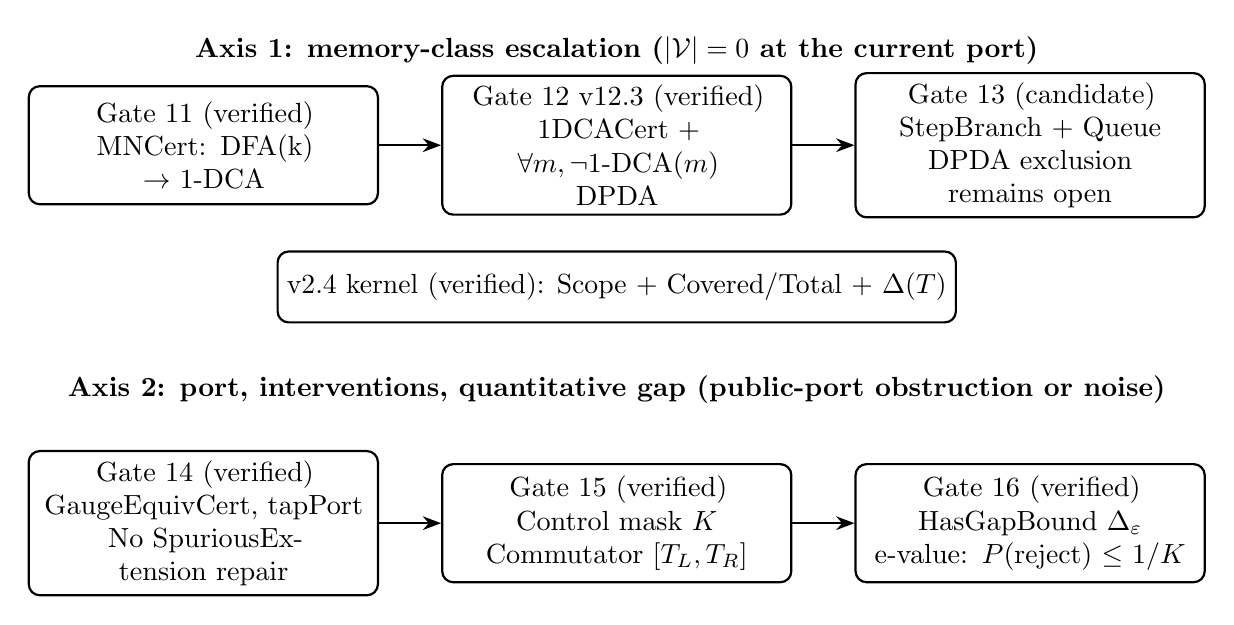
\begin{tikzpicture}[>=Stealth, box/.style={draw,rounded corners,align=center,minimum height=15mm,text width=42mm}, thick]
\node at (5.25,0) {\textbf{Axis 1: memory-class escalation (\(|\mathcal V|=0\) at the current port)}};
\node[box] (a) at (0,-1.2) {Gate 11 (verified)\\MNCert: \mbox{DFA(k)} \(\to\) \mbox{1-DCA}};
\node[box] (b) at (5.25,-1.2) {Gate 12 v12.3 (verified)\\1DCACert + \(\forall m,\neg\mathrm{1\text{-}DCA}(m)\)\\DPDA};
\node[box] (c) at (10.5,-1.2) {Gate 13 (candidate)\\StepBranch + Queue\\DPDA exclusion remains open};
\draw[->] (a)--(b); \draw[->] (b)--(c);
\node[draw,rounded corners,align=center,minimum height=9mm] at (5.25,-3.0) {v2.4 kernel (verified): Scope + Covered/Total + \(\Delta(T)\)};
\node at (5.25,-4.3) {\textbf{Axis 2: port, interventions, quantitative gap (public-port obstruction or noise)}};
\node[box] (d) at (0,-6.0) {Gate 14 (verified)\\GaugeEquivCert, tapPort\\No SpuriousExtension repair};
\node[box] (e) at (5.25,-6.0) {Gate 15 (verified)\\Control mask \(K\)\\Commutator \([T_L,T_R]\)};
\node[box] (f) at (10.5,-6.0) {Gate 16 (verified)\\HasGapBound \(\Delta_\varepsilon\)\\e-value: \(P(\mathrm{reject})\le 1/K\)};
\draw[->] (d)--(e); \draw[->] (e)--(f);
\end{tikzpicture}}
\caption{Two axes of research escalation: Axis 1 changes the memory class when \(|\mathcal V|=0\); Axis 2, verified in Lean 4.36.0, covers escalation of the observation port, intervention algebra, and the quantitative residual gap when a certified public-port obstruction or observation noise is present.}
\end{figure}

\textbf{Theorem 7.1 (Axis 2: port, interventions, and quantitative residual; verified in Lean 4.36.0).} The three independent modules, all written in Lean 4 Core without sorry, establish the following.

\begin{enumerate}
\item \textbf{Gate 14 (gate14\_\allowbreak port\_\allowbreak escalation\_\allowbreak v2\_\allowbreak 4.lean, 10 declarations [4]).} For a two-stage mechanism \(Q\xrightarrow{R}Z\xrightarrow{S}Y\) and an invertible transformation \(T\) (GaugeEquivCert: \(T(R(q_0))\ne R(q_0)\)), the gauge-equivalent counterpart \(M_2=(T\circ R,S\circ T^{-1})\) differs from \(M_1\) but is indistinguishable on any log through publicPort (gaugeCert\_\allowbreak blocks\_\allowbreak single\_\allowbreak port\_\allowbreak id). A port refinement PortRefinement, with the non-strict condition \(\mathrm{proj}\circ P_2=P_1\), preserves earlier refutations. The extended tapPort breaks the gauge equivalence on a single query \(q_0\) (tapPort\_\allowbreak breaks\_\allowbreak gaugeCert). An observationally unproductive SpuriousExtension, whose observable image is unchanged, cannot repair a refuted class on any log (spurious\_\allowbreak extension\_\allowbreak cannot\_\allowbreak repair\_\allowbreak refutation).

\item \textbf{Gate 15 (gate15\_\allowbreak intervention\_\allowbreak algebra\_\allowbreak v2\_\allowbreak 4.lean, 8 declarations [5]).} For two interventions \(T_L,T_R\) under a formal normalizer \(N\), local orthogonality of the mask \(K\) at \(x_0\) is checked by the computable checkOrthogonalControl predicate (by decide). If \(T_L\) globally preserves \(N\), then the commutation relation \(N(T_L(T_R x))=N(T_R(T_L x))\) is equivalent to language invariance of the strategy \(T_R\). A single noncommutation witness refutes joint invariance (noncomm\_\allowbreak refutes\_\allowbreak joint\_\allowbreak invariance). The anti-leakage results confounded\_\allowbreak TL\_\allowbreak fakes\_\allowbreak noncomm\_\allowbreak without\_\allowbreak mask\_\allowbreak K and unaligned\_\allowbreak normalizer\_\allowbreak fakes\_\allowbreak semantic\_\allowbreak shift give two separate counterexamples: violating Held can create order dependence even when the strategy is language-insensitive, while an unaligned \(N\) can create a spurious one-step semantic shift even when the interventions commute.

\item \textbf{Gate 16 (gate16\_\allowbreak stochastic\_\allowbreak gap\_\allowbreak evalue\_\allowbreak v2\_\allowbreak 4.lean, 11 declarations [6]).} On exact discrete measures with natural-number masses, the module proves Markov's inequality (markov\_\allowbreak ineq) and a false-rejection bound for valid e-variables \(\mathbb E_\mu[E/D]\le1\):
\[
K\cdot\mathrm{eventMass}(\mu,\{E\ge KD\})\le\mathrm{totalMass}(\mu)
\]
(evalue\_\allowbreak false\_\allowbreak rejection\_\allowbreak bound). It also establishes validity of the product of two independent e-variables (indep\_\allowbreak two\_\allowbreak step\_\allowbreak evalue\_\allowbreak product\_\allowbreak valid). The quantitative residual gap is
\[
\begin{gathered}
\mathrm{HasGapBound}(\mu,\mathrm{Gap},\mathrm{num},\mathrm{den})\Longleftrightarrow\\
(0<\mathrm{den})\land
\bigl(\mathrm{eventMass}(\mu,\mathrm{Gap})\cdot\mathrm{den}
\le\mathrm{num}\cdot\mathrm{totalMass}(\mu)\bigr).
\end{gathered}
\]
It excludes a vacuous zero denominator (den\_\allowbreak zero\_\allowbreak rejected\_\allowbreak by\_\allowbreak HasGapBound, no axioms), generalizes GapEmpty (gapEmpty\_\allowbreak implies\_\allowbreak zero\_\allowbreak gapBound), and is subadditive for a common denominator (union\_\allowbreak gap\_\allowbreak bound).

\end{enumerate}
\textbf{Meta-synset operators and the conditional Axis 1 \(\leftrightarrow\) Axis 2 fork.} The v2.4 kernel adds the basic MetaOperand structure (with the nondegeneracy invariant \(2\le\mathrm{domainCount}\)), metaProj, metaFreeze (metaFreeze\_\allowbreak preserves\_\allowbreak candidates), and the conditional fork chooseConditionalTwoAxisAction / conditional\_\allowbreak two\_\allowbreak axis\_\allowbreak routing\_\allowbreak blocks\_\allowbreak spurious\_\allowbreak memory\_\allowbreak escalation. Under the postulated incompatibility of causes (disjointCause), gauge nonidentifiability (axis2Gauge) blocks indiscriminate Axis 1 memory escalation. The scope is conditional: axis1Refuted and axis2Gauge are free predicates, not yet derived together in one type from VersionSpaceEmpty and GaugeEquivCert.

\section{Machine verification in Lean 4.36.0 and limits of the results}

Table 1 separates results already verified by the Lean kernel (exit code 0, zero sorryAx) from components that remain specifications, candidates, or open empirical questions.

\begin{table}[htbp]
\caption{Verified modules and open components of the v2.4 architecture (Lean 4.36.0, zero \texttt{sorryAx}).}
\small
\setlength{\tabcolsep}{3pt}
\begin{tabularx}{\linewidth}{@{}>{\raggedright\arraybackslash}p{.16\linewidth}>{\raggedright\arraybackslash}X>{\raggedright\arraybackslash}p{.24\linewidth}>{\raggedright\arraybackslash}p{.24\linewidth}@{}}
\toprule

Layer / module & Key theorems & Lean 4.36.0 axiom dependencies & Actual status \\
\midrule
Revision kernel v2.4 & 15 declarations, including pointwise\_\allowbreak unproved\_\allowbreak blocks\_\allowbreak any\_\allowbreak total, stepBranch\_\allowbreak fails\_\allowbreak without\_\allowbreak injectiveBin, metaFreeze\_\allowbreak preserves\_\allowbreak candidates, conditional\_\allowbreak two\_\allowbreak axis\_\allowbreak routing… & 9 axiom-free; 2 propext; 1 Quot.sound; 3 use the standard trio & Verified [3] (1bb76af2…, 605 lines, 0 warnings) \\
Gate 11–12 v12.3 & 12 theorems: checkMNCert\_\allowbreak sound, check1DCACert\_\allowbreak sound, checkFullChomskyProtocol\_\allowbreak sound & propext, Classical.choice, Quot.sound & Verified [2] (763f59d7…) \\
Gate 14 v2.4 (Port) & 10 declarations, including gaugeCert\_\allowbreak blocks\_\allowbreak single\_\allowbreak port\_\allowbreak id, tapPort\_\allowbreak breaks\_\allowbreak gaugeCert, spurious\_\allowbreak extension\_\allowbreak cannot\_\allowbreak repair\_\allowbreak refutation & 8 axiom-free; 2 propext and Quot.sound & Verified [4] (34397f38…, 272 lines, 0 warnings) \\
Gate 15 v2.4 (Operators) & 8 declarations, including checkNonCommProtocol\_\allowbreak sound, noncomm\_\allowbreak refutes\_\allowbreak joint\_\allowbreak invariance, Held/\(N\) anti-leakage & 5 axiom-free; 3 propext & Verified [5] (67fbae74…, 231 lines, 0 warnings) \\
Gate 16 v2.4 (Gap \(\Delta_\varepsilon\)) & 11 declarations, including markov\_\allowbreak ineq, evalue\_\allowbreak false\_\allowbreak rejection\_\allowbreak bound, indep\_\allowbreak two\_\allowbreak step\_\allowbreak evalue\_\allowbreak product\_\allowbreak valid, den\_\allowbreak zero\_\allowbreak rejected\_\allowbreak by\_\allowbreak HasGapBound & 1 axiom-free; 3 propext; 7 propext and Quot.sound & Verified [6] (9cf958f2…, 304 lines, 0 warnings) \\
Gate 13 (Level 4) & QueueProgram; \(\forall m,\neg\mathrm{StackProgram}(m)\) & — & Candidate (Lean run pending) \\
Empirical transfer & Full-cost gain from StepBranch and meta-synset & — & Open hypothesis (benchmark planned) \\
\bottomrule
\end{tabularx}
\end{table}
\textbf{Remark 8.1 (Exact scope of v2.4 after the formal audit).}

\begin{enumerate}
\item \textbf{Gate 14.} PortRefinement expresses a non-strict refinement (\(\mathrm{proj}\circ P_2=P_1\)); strict escalation is established separately by tapPort\_\allowbreak breaks\_\allowbreak gaugeCert. The sameObs condition in SpuriousExtension is assumed for all \(f:Q\to O\), not inferred syntactically from the grammar.
\item \textbf{Gate 15.} Orthogonality of the control mask \(K\) is checked locally at a specified \(x_0\). The confounding results are existential: violating Held can create misleading order dependence, and misaligning \(N\) can create a spurious semantic shift.
\item \textbf{Gate 16 v2.4.} The condition \(0<\mathrm{den}\) is part of the HasGapBound definition and is confirmed by den\_\allowbreak zero\_\allowbreak rejected\_\allowbreak by\_\allowbreak HasGapBound. A probabilistic interpretation additionally requires \(\mathrm{totalMass}(\mu)>0\), since the current definition does not exclude the zero measure. The union\_\allowbreak gap\_\allowbreak bound rule uses a common denominator \(q\). The indep\_\allowbreak two\_\allowbreak step\_\allowbreak evalue\_\allowbreak product\_\allowbreak valid theorem proves a product for a fixed pair of steps, not arbitrary data-dependent stopping (Ville's theorem).
\item \textbf{Kernel v2.4.} All four modules compile without warnings in ALL\_\allowbreak 4\_\allowbreak MODULES\_\allowbreak v2\_\allowbreak 4\_\allowbreak VERIFICATION.log. The conditional\_\allowbreak two\_\allowbreak axis\_\allowbreak routing… result nevertheless remains a conditional fork based on postulated disjointCause over free predicates axis1Refuted and axis2Gauge. If both predicates are false, its default branch returns Axis 2, because a separate InsufficientEvidence outcome is deferred to the next version's unified controller. metaFreeze carries the candidate list and the log prefix, but not yet a complete gap and provenance certificate. In gate12\_\allowbreak 13\_\allowbreak parametric\_\allowbreak lift, hPart takes a True \(\to\) premise throughout \(Q_{\rm mod}\); in pointwise\_\allowbreak unproved\_\allowbreak blocks\_\allowbreak any\_\allowbreak total, nonexistence is proved for total justifications satisfying the exact scope equality \(\mathrm{tot}.R=R\).

\end{enumerate}
\section{Conclusion}

In v2.4 the dual pair meta-synset \(\leftrightarrow\) invariant covers both axes of research escalation. The 44 machine-verified Lean 4.36.0 declarations cover the v2.4 revision kernel, escalation of the observation port (Gate 14), an intervention algebra with a computable mask \(K\) (Gate 15), and a quantitative residual gap with exact e-value bounds (Gate 16). The central objects are sealed evidence DirectEvidence s A c; the mandatory residual gap \(\Delta(T)\), with its covering proof partition; the distinction between the completion bridge bridgeComplete and the cross-scope lift liftScope; the dependent inference license \(\Gamma(\kappa)\); and branching selection within \(R\), with the prerequisites encoded by SymbolLift. The two immediate next steps are local verification of Level 4 (Gate 13, QueueProgram) and a full-cost comparison of the branching StepBranch controller with linear escalation on held-out tasks.

\begin{thebibliography}{15}
\bibitem{ref1} A. Strand. \emph{Meta-Synset II: Certified Revision of the Hypothesis Language. Typed Transfer, Scope of Inference, and Verifiable Representational Change}. v0.3, manuscript, 2026.
\bibitem{ref2} A. Strand. \emph{Hypothesis Languages and Proof-Based Representational Escalation: From Finite Impossibility Certificates to Parametric Theorems on Counter and Stack Automata}. Gate 11–12 v12.3, 2026.
\bibitem{ref3} A. Strand. epistemic\_\allowbreak revision\_\allowbreak kernel\_\allowbreak v2\_\allowbreak 4.lean: Formal kernel of the v2.4 revision system. Lean 4.36.0, SHA-256 1bb76af2f6cc0334\allowbreak 8fa35e605d6ce41d\allowbreak fbd35cfcb9f5ae2a\allowbreak 0ec8491c792319c7, 15 declarations, 0 warnings, 2026.
\bibitem{ref4} A. Strand. gate14\_\allowbreak port\_\allowbreak escalation\_\allowbreak v2\_\allowbreak 4.lean: Escalation of the observation port and exclusion of unproductive extensions. Lean 4.36.0, SHA-256 34397f3839bcc9cd\allowbreak b06335b1ca959e2f\allowbreak 983dbad1635edf74\allowbreak 30cb7d767e0ddcc6, 10 declarations, 0 warnings, 2026.
\bibitem{ref5} A. Strand. gate15\_\allowbreak intervention\_\allowbreak algebra\_\allowbreak v2\_\allowbreak 4.lean: Intervention algebra, a local computable mask \(K\), and the commutator \([T_L,T_R]\). Lean 4.36.0, SHA-256 67fbae749cc0ab16\allowbreak 3468879396bca8e6\allowbreak f14f38f881ef63b7\allowbreak 8119888c4bad9c22, 8 declarations, 0 warnings, 2026.
\bibitem{ref6} A. Strand. gate16\_\allowbreak stochastic\_\allowbreak gap\_\allowbreak evalue\_\allowbreak v2\_\allowbreak 4.lean: Quantitative residual gap \(\Delta_\varepsilon\) with \(0<\mathrm{den}\) and product of two independent e-values. Lean 4.36.0, SHA-256 9cf958f26f67e411\allowbreak 2367090ff5fbbcd8\allowbreak 95dcf9db84988649\allowbreak 4164a2b9fc640d99, 11 declarations, 0 warnings, 2026.
\bibitem{ref7} D. Gentner. Structure-Mapping: A Theoretical Framework for Analogy. \emph{Cognitive Science}, 7:155–170, 1983.
\bibitem{ref8} J. A. Goguen and R. M. Burstall. Institutions: Abstract Model Theory for Specification and Programming. \emph{Journal of the ACM}, 39(1):95–146, 1992.
\bibitem{ref9} D. Blackwell. Equivalent Comparisons of Experiments. \emph{Annals of Mathematical Statistics}, 24(2):265–272, 1953.
\bibitem{ref10} D. Angluin. Learning Regular Sets from Queries and Counterexamples. \emph{Information and Computation}, 75(2):87–106, 1987.
\bibitem{ref11} J. Myhill. \emph{Finite Automata and the Representation of Events}. WADC Technical Report 57–624, 1957.
\bibitem{ref12} A. Nerode. Linear Automaton Transformations. \emph{Proceedings of the American Mathematical Society}, 9(4):541–544, 1958.
\bibitem{ref13} I. Lakatos. \emph{Proofs and Refutations: The Logic of Mathematical Discovery}. Cambridge University Press, 1976.
\bibitem{ref14} B. Huffman and O. Kunčar. Lifting and Transfer: A Modular Design for Quotients. \emph{CPP 2013}, LNCS 8307, 131–146, 2013.
\bibitem{ref15} S. Jha and S. A. Seshia. A Theory of Formal Synthesis via Inductive Learning. \emph{Acta Informatica}, 54:693–726, 2017.
\end{thebibliography}
\end{document}
